\documentclass[12pt]{article}
\pdfminorversion=7

% Standard packages for figures, citations, math, tables, etc.
% Feel free to add more as needed!
\usepackage{amssymb}
\usepackage{graphicx}
\usepackage{cite}
\usepackage[cmex10]{amsmath}
\interdisplaylinepenalty=2500 
\usepackage{mdwmath}
\usepackage{mdwtab}
\usepackage{color}
\usepackage{pgfplots}
\usepackage{multirow}
\usepackage{subcaption}
\usepackage{verbatim}
\usepackage{enumitem}
\usepackage{appendix}
\usepackage[outdir=./]{epstopdf}
\usepackage{indentfirst}
\pgfplotsset{compat=1.17}

% Packages for formatting with 1 in margins
\usepackage[latin1]{inputenc}
\usepackage[left=1in,top=1in,right=1in,bottom=1in,nohead]{geometry}
\usepackage{setspace}
\setstretch{1.15}
\setlength\parindent{1cm}

% Define the location of your figures in order to avoid writing absolute file location
\graphicspath{{figures/}}	

\begin{document}

% Title Page
\begin{titlepage}
\begin{center}
{\LARGE \textsc{ECE 445: Senior Design Laboratory} \\ \vspace{8pt}}
\rule[13pt]{\textwidth}{1pt} \\ \vspace{120pt}
{\huge \textbf{\textsc{The Odds Booster}} \\ \vspace{8pt}}
{\LARGE \textbf{\textsc{Design Document}} \\ \vspace{30pt}} 
{\large \textit{Authors:} Marco Rojas \\ \vspace{4pt}
\hspace{48pt} Jack Arndt \\ \vspace{4pt}
\hspace{48pt} Tim Green \\ \vspace{4pt}
\hspace{8pt} \textit{Date Written:} February 20th, 2022}
\vfill
\end{center}

% Numbered pages on everything but title
\pagenumbering{arabic}	
\end{titlepage}
\setcounter{page}{2}

% Introduction can be kept the same as the proposal (same idea from rubric)
\section{Introduction}

Before heading to the casino, individuals need to assess how much money they are willing to lose, since, as the saying goes, ``The house always wins''. Or do they? Is there potentially a way to bring the casino games to the comfort of your home and train/optimize your strategies to ask a different question, ``How much money should I win?''

The Odds Booster is an automated casino game assistant designed to help players learn and manage casino games such as Blackjack or Texas Hold'em. The kit involves a central communicable device along with a custom deck of cards which will be used to determine the best possible move for each player along with the outcome of each hand of the game. This device is an innovation as it brings both the ease and simplicity as well as the ability to learn the game that can be provided by a virtual game into the superior enjoyment and atmosphere of a physical game. Digital poker tables that provide a similar experience exist but cost thousands of dollars. Our design achieves this functionality without an expensive custom table and while allowing for physical cards and chips.

The Odds Booster central device will serve as the hub used by the dealer and all players of the game. The dealer will swipe each card being distributed to the players over the central device and said device will determine the specific card being dealt using an RFID sensor and thin passive RFID tags placed on the cards. This central device will also contain a display detailing the next actions and outcomes for each hand of the game helping each player and the dealer learn the rules of the game. This main device will be paired via Bluetooth to a user's phone app. The card information will be shared with the app and the app will tell the player the strength of their hand or what move will have the best outcome within the context of the game. It is important to note that knowledge of the hands of the other players within the game provides an unfair advantage to the user and such information will be ignored when determining moves for the user. The ethics of the game will be discussed further later in this proposal. The device itself will be battery powered and rechargeable for easy use and mobility. The usage of the device is portrayed in the diagram shown in Figure \ref{fig:use_dia}.

\begin{figure}[h!]
	\centering
	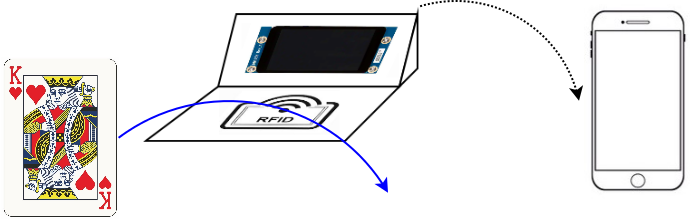
\includegraphics[width=0.9\textwidth]{ProposalUsageDiagram.png}
	\caption{System Usage Diagram}
	\label{fig:use_dia}
\end{figure}

\noindent
The main requirements to ensure the completion and success of this project are as follows.
\begin{itemize}
\item The central device must be able to sense and distinguish the 52 different RFID tags associated with each card.
\item The central device must be able to display the card and game information for all players to see as well as send the information to a phone app via Bluetooth.
\item The phone app must be able to receive game information via Bluetooth and use the information to determine the strength of the user's hand and/or the best possible move for the user.
\end{itemize}
These requirements are broken into more detailed and subsystem specific requirements through the remainder of this proposal.

% Design parts have same structure
\section{Design}

The block diagram describing each subsystem within the system and their connections is shown in Appendix A. The schematic showing the communication subsystem, the display subsystem, and the card reader subsystem is shown in Appendix B. The schematic showing the power subsystem is shown in Appendix C. The design is composed of five main subsystems. Four of the subsystems are outlined by hardware components and labeled in the block diagram. The fifth subsystem is the phone app. The purpose, interconnections, and requirements of each subsystem are described in detail through this section. 

% Each subsystem needs detailed purpose and description, table of parts used for it, circuit schematics, simulations, calculations, coding flow charts, etc.
% Each subsystem also needs an Requirements & Verification table
\subsection{Power Subsystem}

The power subsystem is made up of a rechargeable battery, ESD protection circuitry, a battery management system capable of overvoltage, undervoltage, and overcurrent detection, a voltage regulator, and a boost converter. This subsystem is responsible for providing power to all other hardware components within the system in a safe manner. Without this subsystem, none of the main requirements could be met as each operation of the system requires power. The power subsystem connects to the other three hardware subsystems (the card reader, display, and communication subsystems) via a 3.3V DC voltage used for logic powering provided by the voltage regulator. The power subsystem connects to the display subsystem through an additional 9.6V DC voltage used for the LED backlighting of the LCD display. The battery management system also connects to the communication subsystem as it provides the microcontroller with battery status information in the form of an analog current measurement used for SOC approximation. This signal is used to tell the users important system information such as when the battery is low.

The rechargeable battery will be a lithium ion battery. This is a popular rechargeable battery that tends to have  good energy and power density. More research will be needed on expected power draw to determine the battery capacity sizing. The lithium ion battery output will be connected to a battery management system. The battery management system (BMS) is used to monitor the status of the battery in terms of output voltage and current draw. This protects the battery from being over or undercharged and from being overdrawn by being able to cut power connections. This allows for a longer battery life and a safer device. The BMS is then connected to the voltage regulator. The voltage regulator ensures the voltage of the battery remains at a safe level for each component in the system.

The power subsystem has a set of basic requirements that ensure its proper operation. These requirements are as follows.

\begin{itemize}
\item The battery management system must be able to measure the output voltage of the lithium ion battery to a tolerance of $\pm0.1V$.
\item The battery management system must be able to measure the current in or out of the lithium ion battery to a tolerance of $\pm10mA$.
\item The battery management system must be able to disconnect connected components if the lithium ion battery voltage falls too low or moves too high (specific boundaries depend on specific battery model safety specifications).
\item The voltage regulator must be able to maintain a voltage within a safe range of $3.1V$ to $3.5V$ (safe operating range for average CMOS device \cite{TI_inverter}).
\item The power must be able to continuously provide at least $500mA$ given the voltage regulator requirements
\end{itemize}

\subsection{Communication Subsystem}

The communication subsystem is made up of the Bluetooth transceiver, 2.4GHz antenna and the microcontroller. These components are combined into a single module which can be used as the central microcontroller within the device. The reasoning for using a single module is explained next. This subsystem is responsible for communicating the card and game data from the central device to the phone app as well as receiving information from the phone app. The subsystem is vital for the second and third main requirements in sending the game data and allowing the use of this data within the phone app. The communication subsystem connects to the power subsystem through the 3.3V DC supply provided by the voltage regulator of the power system, to the card reader subsystem through the transfer of card data through an SPI interface to the microcontroller, and to the phone app through a 2.4GHz Bluetooth v4.2 wireless signal provided by the internal antenna.

This subsystem has been adjusted from previous plans to be consolidated within a single purchasable component. The component chosen for this purpose is the ESP32-WROVER-E module (henceforth referred to as the MCU module) which combines a microcontroller, flash memory, DRAM, and 2.4GHz antenna into a single surface-mount component. This simplifies the design of the communications subsystem by allowing the Bluetooth packets and connections to be initiated by the built-in Bluetooth protocol and API of the microcontroller, rather than communicated through a serial communication protocol to a new chip to do the same operations. This also prevents the design of high frequency RF traces and discrete matching networks on our PCB to connect the Bluetooth transceiver component to an external antenna. Traces at such a frequency can be heavily affected by tolerances of the PCB manufacturing leading to poor performance as compared to a combined module with guaranteed operation specifications as chosen here. Lastly, the combined module is well documented allowing for a faster development process in getting a functioning connection between this device and a phone app allowing for more focus on other hardware components.

The MCU module is shared by other subsystems requiring embedded C code to function properly and as such the design requirements and reasoning for this device are split among the subsystem descriptions. For the communication subsystem, the MCU module provides an API for generating Bluetooth v4.2, a low power alternative to classic Bluetooth ideal for battery powered devices with a low required throughput such as this device. As previously mentioned, the MCU module provides a 2.4GHz antenna to transmit the Bluetooth packets making this module an ideal choice. The module also has an associated low-cost development kit (ESP-DEVKITC-VE) allowing for easy coding and troubleshooting before programming to our finished board.

The communication subsystem is included within the schematic shown in Appendix B. The subsystem does not require an individual schematic as it is solely comprised of the MCU module and programming circuitry, and the MCU module is shared between multiple subsystems. The reset button shown is used to boot the device. A simple RC circuit with a time constant of $\tau = RC = 1ms$ is applied after the push button to provide debouncing and avoid multiple resets from a single press. The simulation of this reset button being pressed is shown below in Figure \ref{fig:reset_debounce}. The boot switch is a programming feature as this switch controls if the microcontroller downloads a program through the UART interface on boot (IO0 = low), or if the microcontroller uses the saved program from the flash memory for its instructions (IO0 = high). The boot control also relies on the IO2 pin being low on boot and has been connected to a pull-down resistor for this reason. Simple breakout pins will be included (as shown in the schematic) to connect to a UART interface for programming the microcontroller.

The communication module requires significant software control. A flow diagram explaining the function of the microcontroller firmware is provided in Appendix D as this code also controls aspects of other modules.

\begin{figure}[h!]
	\centering
	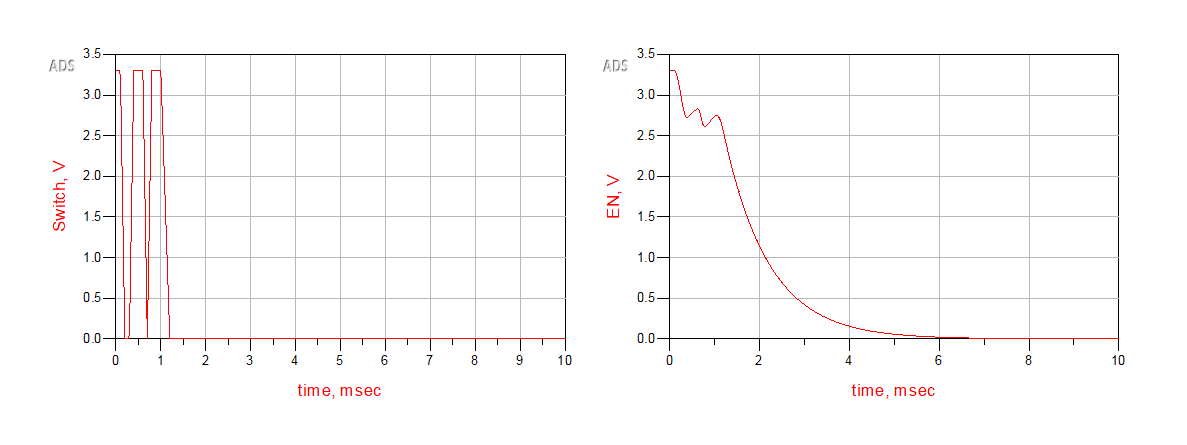
\includegraphics[width=0.9\textwidth]{reset_debounce.png}
	\caption{Reset Button Debounce Simulations}
	\label{fig:reset_debounce}
\end{figure}

The requirements and validation methods for the communication subsystem that ensure its proper operation are shown in Table \ref{tab:comms_rv} Notice that there are no requirements for latency of information transmission. As this device is sending very low amounts of information and the actions are not time sensitive, latency is not included as a requirement.

\begin{table}[h!]
	\caption{Communication Subsystem Requirements and Verification}
	\label{tab:comms_rv}
	\centering
	\begin{tabular}{| p{0.45\linewidth} | p{0.45\linewidth} |} 
 		\hline
 		\textbf{Requirements} & \textbf{Verification} \\ 
 		\hline
 		\begin{enumerate}
 			\item The communication subsystem must use Bluetooth v4.2 \cite{IEEE_bt} to transmit and receive information to and from the phone app at a distance of 3ft with an average throughput of 10kbps.
		\end{enumerate} & \begin{enumerate}[label=\alph*)]
 			\item Somin
		\end{enumerate} \\
 		\hline
	\end{tabular}
\end{table}

\subsection{Card Reader Subsystem}

The card reader subsystem is made up of the microcontroller and the RFID sensor. The subsystem is responsible for reading the card ID of each card swiped past the device. The subsystem is vital for the first main requirement of sensing and distinguishing each of the 52 cards. The card reader subsystem connects to the power subsystem through the provided $3.3V_{DC}$ supply, and to the communication subsystem through the passing of card data through an SPI interface to the microcontroller.

The RFID sensor generates a specific frequency signal that powers the RFID tags on the cards and results in the cards transmitting a signal containing the serial ID of the tag. The frequency of the sensor depends on the selected RFID tags operating frequency. The microcontroller is shared by multiple subsystems but will receive this serial ID from the sensor via wired serial transmission.

The basic requirements for the card reader subsystem that ensure its proper operation are as follows.

\begin{itemize}
\item The RFID sensor must be able to accurately determine the serial ID of an RFID tag when held to the surface of the sensor.
\item The microcontroller must be able to accurately receive the serial ID of the RFID tag when serially transmitted from the RFID sensor.
\end{itemize} 

\subsection{Display Subsystem}

The display subsystem is made up of the microcontroller and the display. The subsystem is responsible for showing the user the game actions and current game information. The subsystem is vital for the second main requirement in displaying to the players and dealer the game status and next actions. The game status display subsystem connects to the power subsystem through the 3.3V DC logic supply and 9.6V DC LED backlight supply, and the card reader subsystem through the transfer of card data via SPI interface to the microcontroller.

The LCD display within the subsystem is an output device showing the video data provided to it by the microcontroller. The LCD display chosen receives input data through a parallel 24bit RGB input. This input method requires a large number of GPIOs from the microcontroller which is not convenient for any hand-soldering based projects\footnote{Many microcontrollers with a large number of GPIOs come in BGA (Ball Grid Array) packaging or QFP/QFN (Quad Flat Packaging with or without leads) packaging with a very small pin pitch. These packaging formats are very hard to solder with only a hand soldering iron.}. Alternative displays with fewer pins exist that use protocols such as MIPI DSI, but this protocol is not publicly available and requires significant work to design a functioning interface. To handle this issue, high frequency shift registers are used for each color channel. The shift register has a serial input and 8-bit parallel output allowing for the use of three GPIOs to define each pixel color instead of 24 given the microcontroller can generate output signals at a rate at least eight times the specified clock signal.

The chosen components meet these design requirements as the $320\times240$ pixel LCD specifies a typical data clock frequency of $6.5MHz$. This screen size requires a $230.4kB$ of memory for a full screen buffer. The MCU module can utilize clocks up to $160MHz$ for LCD control (much larger than eight times the LCD clock requirement) and can output up to three clock signals allowing for the control of both the LCD data clock ($6.5MHz$) and faster shift register clocks ($52MHz$). The chosen MCU module also has a large amount of included memory external to the microcontroller. An $8MB$ PSRAM unit is included within the module providing plenty of space for frame buffers. This memory can be accessed at a rate of up to $80MHz$ with up to 32-bit reads and writes. This data size and access rate far exceeds the requirements set by the LCD allowing for efficient and easy writing reading from a potential double-buffered display. An additional level of redundancy is added with included internal memory components. The MCU includes 520kB of internal SRAM to be used in the case of the external PSRAM unit failing to meet the application needs for any reason.

The connections between the LCD, shift registers, and MCU module are shown in the schematic in Appendix B. The LCD control is controlled by firmware and thus is included within the flow diagram shown in Appendix D.

The requirements and verification methods for the display subsystem that ensure its proper operation are shown below in Table \ref{tab:display_rv}

\begin{table}[h!]
	\caption{Display Subsystem Requirements and Verification}
	\label{tab:display_rv}
	\centering
	\begin{tabular}{| p{0.45\linewidth} | p{0.45\linewidth} |} 
 		\hline
 		\textbf{Requirements} & \textbf{Verification} \\ 
 		\hline
 		\begin{enumerate}
 			\item The microcontroller must generate both 6.5MHz ($\pm 0.1MHz$) and 52MHz ($\pm 1MHz$) clock signals simultaneously through its clock output pins.
		\end{enumerate} & \begin{enumerate}[label=\alph*)]
 			\item Connect the ESP32-WROVER-E module to a 3.3V power supply. 
 			\item Program the MCU in download mode using the UART interface and set the GPIO control registers to have CLK\_OUT2 at pin 35 and CLK\_OUT3 at pin 34 with frequencies 52MHz and 6.5MHz respectively. 
 			\item Connect these pins to separate channels of an oscilloscope. Use the frequency analysis features of the oscilloscope to record the frequency of each output signal .
		\end{enumerate} \\
		\hline
		\begin{enumerate}
		\setcounter{enumi}{1}
 			\item The microcontroller must output the screen data serially to the three specified GPIO pins with a clock rate of 52MHz.
		\end{enumerate} & \begin{enumerate}[label=\alph*)]
 			\item A
		\end{enumerate} \\
		\hline
		\begin{enumerate}
		\setcounter{enumi}{2}
 			\item The microcontroller must write to external PSRAM to update displayed screen data while display is active.
		\end{enumerate} & \begin{enumerate}[label=\alph*)]
 			\item A
		\end{enumerate} \\
 		\hline
	\end{tabular}
\end{table}

\subsection{Phone App Subsystem}

The phone app subsystem is made up of solely the application used by the phone. The subsystem is responsible for receiving the communications from the central device and sending control information back to the device. The subsystem is vital for the third main requirement in the receipt of game data by the phone and display of optimal moves or game statistics. The phone app subsystem connects only to the communication subsystem through the Bluetooth transmission of game information.

The phone app relies on the device having Bluetooth capabilities. Most modern devices have such capabilities so this should not be a difficult requirement to meet. Android devices are slightly easier to develop with since Android studio and development information is open to the public, therefore the phone app will be developed initially for an Android device using Android Studio.

The app receives game data from the communications system through Bluetooth packets. The app then uses the information of the cards within the player's hand and all other cards showing on the board and uses to determine the strength of the users hand in relation to other possible hands in the current scenario. The strength measurement is calculated as the hand percentile indicating the percentage of currently possible hands against which the user's hand will win. The app displays this strength measurement to the user and will use it to suggest moves to the user. As a baseline, this suggestion will be implemented off a measurement threshold where higher strength measurements lead to more aggressive moves (betting) and lower measurements lead to less aggressive moves (folding). With enough time and successful work, the app could potentially use a deep network model to continue to provide better suggestions with more use.

The app will also be able to provide control information to the central device. The phone app will set the game type and the number of players within the game. This information is important to the functionality of the display module to provide the correct actions of for the dealer/players. The phone app will also be able to reset the hand in the case of a dealing issue. 

The basic requirements for the phone app subsystem that ensure its proper operation are shown in Table \ref{tab:app_rv}.

\begin{table}[h!]
	\caption{Phone App Subsystem Requirements and Verification}
	\label{tab:app_rv}
	\centering
	\begin{tabular}{| p{0.45\linewidth} | p{0.45\linewidth} |} 
 		\hline
 		\textbf{Requirements} & \textbf{Verification} \\ 
 		\hline
 		\begin{enumerate}
 			\item The app will utilize the Bluetooth capabilities of the device to send and receive data with the central device.
		\end{enumerate} & \begin{enumerate}[label=\alph*)]
 			\item A
		\end{enumerate} \\
		\hline
		\begin{enumerate}
		\setcounter{enumi}{1}
 			\item The app will use card information to accurately calculate the ``strength'' measure or the percent of possible alternate hands against which the user's hand will win.
		\end{enumerate} & \begin{enumerate}[label=\alph*)]
 			\item A
		\end{enumerate} \\
		\hline
		\begin{enumerate}
		\setcounter{enumi}{2}
 			\item The app will display the measures and suggestions in the form of text for the user.
		\end{enumerate} & \begin{enumerate}[label=\alph*)]
 			\item A
		\end{enumerate} \\
 		\hline
	\end{tabular}
\end{table}

% Tolerance analysis for the hardest part of the design (most likely to fail or cause problems)
\subsection{Tolerance Analysis}

\section{Cost and Schedule}

\subsection{Cost Analysis}

% table holds any purchasble parts and (if they serve as a block within the block diagram) the block label they correspond with
\begin{table}[h!]
	\caption{Bill of Materials}
	\label{tab:block_comps}
	\centering
	\begin{tabular}{ |c|c|c| } 
 		\hline
 		\textbf{Component Name} & \textbf{Quantity} & \textbf{Total Cost} ($\$$) \\
 		\hline
 		\multicolumn{3}{|c|}{Power Subsystem} \\
 		\hline
 		
 		\hline
 		\multicolumn{3}{|c|}{Communication Subsystem} \\
 		\hline
 		ESP32-WROVER-E & 2 & 7.20 \\
 		ESP32-DEVKITC-VE & 1 & 11.00 \\
 		Paialu CP2102 USB to UART Interface & 1 & 8.76 \\
 		10k 0805 Resistor & 6 & 0.90 \\
 		0.1u 0805 Capacitor & 2 & 0.30 \\
 		\hline
 		\multicolumn{3}{|c|}{Card Reader Subsystem} \\
 		\hline
 		
 		\hline
 		\multicolumn{3}{|c|}{Display Subsystem} \\
 		\hline
 		Orient Display AFY320240A0-3.5N6NTN-R & 1 & 11.53 \\
 		Hirose FH40-40S-0.5SV Connector & 2 & 5.50 \\
 		Nexperia 74LV164D Shift Register & 5 & 2.15 \\
 		\hline
	\end{tabular}
\end{table}

\subsection{Schedule}

\section{Ethics and Safety}

Gambling and wagering money on casino games inherently raises an ethics-eyebrow. Getting involved in this space requires the ability to tread lightly and ensure the IEEE Code of Ethics \cite{IEEE_ethics} is followed to a tee. While our project is aimed at improving players' abilities to perform in the casino, there are measures that need to be accounted for during the development of this project and issues that could potentially arise from accidental or intentional misuse of our project. 

First, we must acknowledge what are the common laws that are broken when cheating in the casino. NRS 465.083 \cite{NRS}, according to Nevada law, prohibits players from cheating at a casino game, which by definition is the manipulation of the outcome of the game or the payments made. This can lead to a felony charge, with 1 to 5 years in prison, restitution, and up to \$10,000 in fines. Essentially, this is a fraud charge specifically citing it happening in the casino. The legal definition is stated as ``alter[ing] the elements of chance, method of selection, or criteria which determine'' the results, amount of payment, or frequency of payment in a game \cite{NRS}; This relates to IEEE Code of Ethics I.4 \cite{IEEE_ethics}. In order to avoid ethical breaches, we are requiring that the usage of our project will have all casino cards scanned and in need of compliance with the dealer. Any dealer that is sitting at a table game in the casino will clearly not agree to use our project as it's in clear violation of casino policy, and even with a dealer that is in cahoots with the player will immediately be caught with the ``Eyes in the Sky'' which is the term for the security measures in the casino. Essentially, we are taking the route that there is no secretive way to use this device in the casino that you wouldn't get caught trying to use outside resources to help boost your odds and chances of winning. A custom deck of cards and a table-top card scanner is impossible to get by the security systems at the casino. 

Next, we look into the potential harm that this project can deliver to the players and general public. This relates to IEEE Code of Ethics I.1 \cite{IEEE_ethics}, and due to our planned usage of RFID and Bluetooth technologies, we are not transmitting or receiving any harmful signals that are outside the typical broadband spectrum of frequencies. There will be no cause of concern for the wireless communications occurring throughout the usage of this project. According to the FDA, there is no evidence of any adverse effects associated with the usage of passive RFID \cite{FDA_RFID}.

Furthermore, IEEE Code of Ethics I.3 \cite{IEEE_ethics} references conflicts of interest, which could potentially pertain to the casinos and their disliking to players increasing their odds of winning. Since this is purely an educational tool, there should be no issues with the casinos and the usage of this in the casino proper is virtually impossible thanks to our design of the project and tight security measures that are relevant to every casino.

Since our project does not in any way put others down or engage in any sort of harassment or discrimination, the IEEE Code of Ethics II \cite{IEEE_ethics} is fulfilled as well. 

Lastly, taking a quick look at the Bluetooth Code of Conduct \cite{BT_conduct} will show that we are following each item and staying true to the ethics laid out. We are not violating any law, transmitting harmful content or tampering, or sending excessively high volume data transfers or bandwidth consumption.

Ethical breaches are primarily prevented due to the design of our project, which requires the usage of a table-top card scanner and our own custom deck of cards (which obviously can not be used in the casino). Players are unable to use the Odds Booster if the custom deck of cards isn't being used, since it's the way that players are able to know what the best possible choices are to take in the casino games. The card scanner needs to send the information to the phone app to crunch the data, thereby preventing the use of any other cards. 

As with any design project, there will always be safety concerns that need to be acknowledged, assessed, and accounted for. In the following section, these concerns are discussed with respect to their associated hazards and potential solutions to minimize any possibilities of risk.

Typically, the primary point of safety concern for any electrical system design stems from the source of power. The power source is not only responsible for the system's overall functionality, but can also work to destroy necessary hardware components (or subsystems) due to unanticipated variations in power output. To take this into account, our power subsystem consists of a rechargeable battery, a battery management system, and a voltage regulator. As specified in greater detail in the power subsystem section, the battery management system and voltage regulator ensure the system's overall immunity to variations in current and voltage such that each individual component can operate at a safe level. It is important to note that the rechargeable battery being used is a lithium ion battery. As per the ECE 445 Safety Guidelines \cite{445_safety}, ``Any group charging or utilizing certain battery chemistries must read, understand, and follow guidelines for safe battery usage.'' All members of the group have read and agreed to follow the course staff's guidance regarding high capacity batteries \cite{Li_safety} and will complete all necessary safety training and adhere to the guidelines set forth in the aforementioned document. 

Before moving on, it is worth to note that the maximum voltage our system will operate under is approximately 3.3V - 3.6V. Inherently, we will be working with relatively low voltages and currents. This is reassuring to know that while we may not be as subject to the greater (and more dangerous!) risks posed from working with higher voltage equipment, that does not mean we can neglect basic lab and equipment safety policies and procedures. All members of the group have also completed the required lab safety training to gain access to the lab. 

Overall, this project is considered relatively ``safe'' under the context of adhering to proper safety policies and protocols when in the lab. There are no true significant safety concerns to the end user as well. The user will simply operate the device primarily from his/her phone and be isolated from any true risk of electrical or mechanical interaction as the entire system will be housed in a custom CAD-designed enclosure. This enclosure serves a double purpose in that it will shield the user/environment from exposure to the electrical components and vice versa. 

% Bibliography (references in separate file)
\bibliographystyle{IEEEtran}
\bibliography{references.bib}

% Appendix
\newpage
\section{Appendix A: Device Block Diagram}

\begin{figure}[h!]
	\centering
	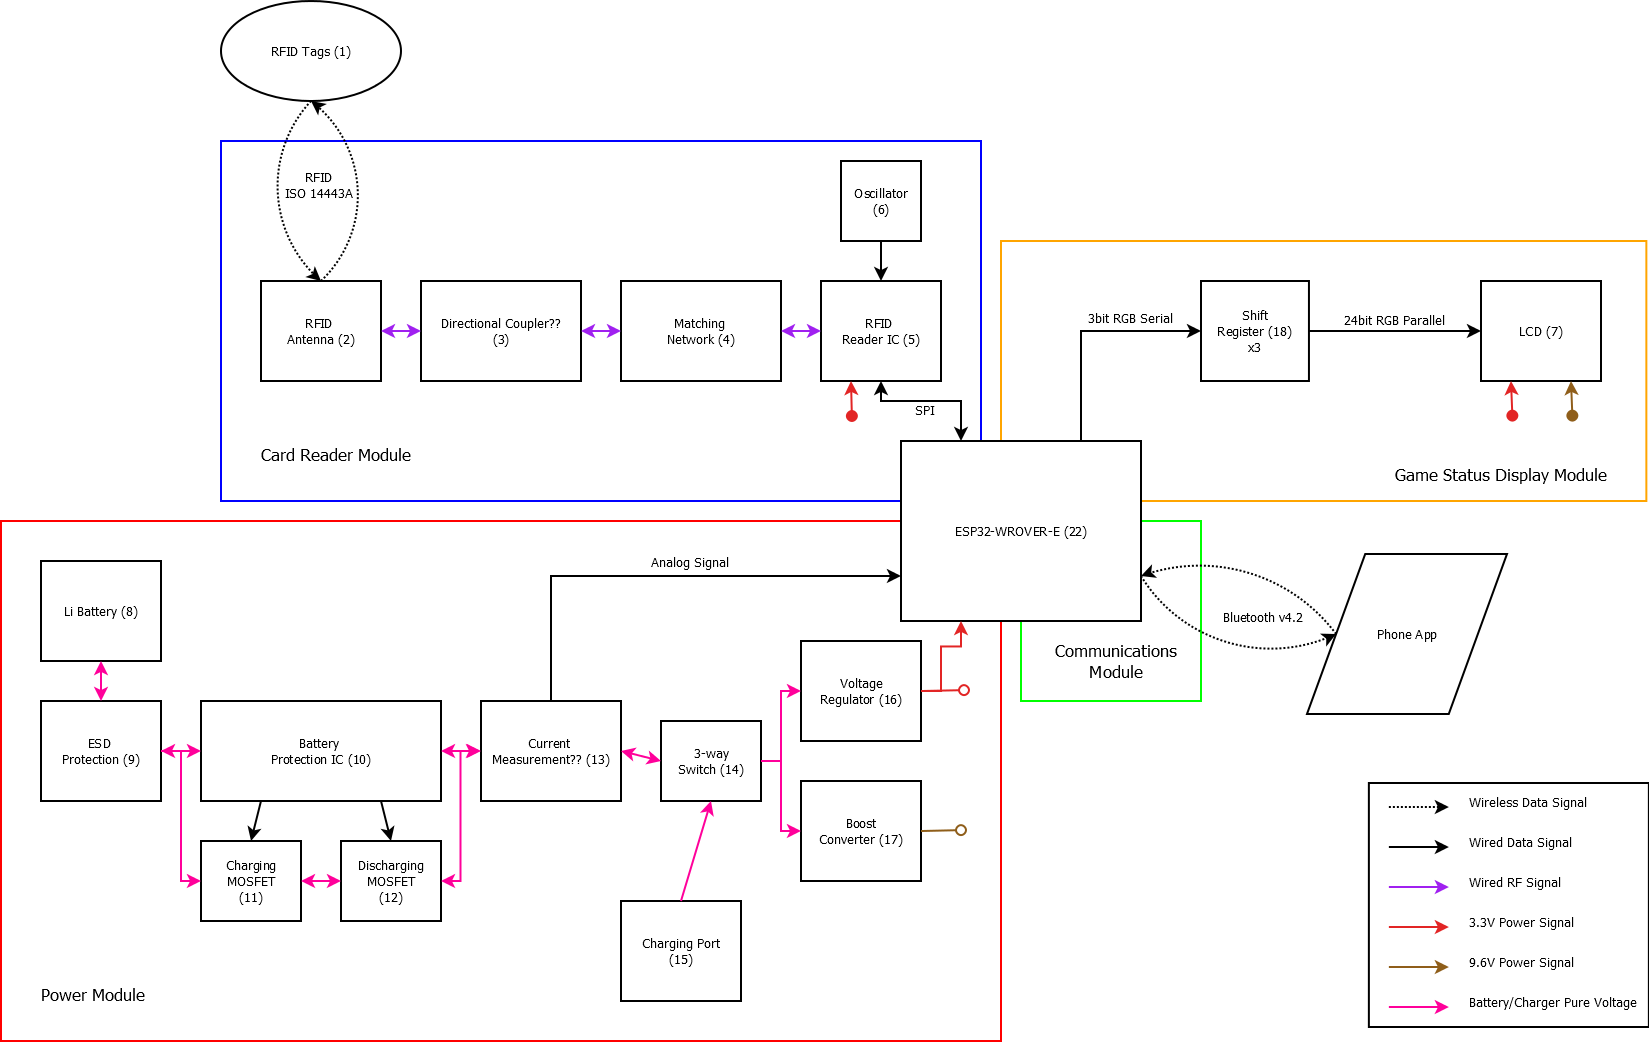
\includegraphics[height=0.93\textheight]{Full_Block_Diagram_v5.png}
\end{figure}

\newpage
\section{Appendix B: Communications and Display Subsystems Schematic}

\begin{figure}[h!]
	\centering
	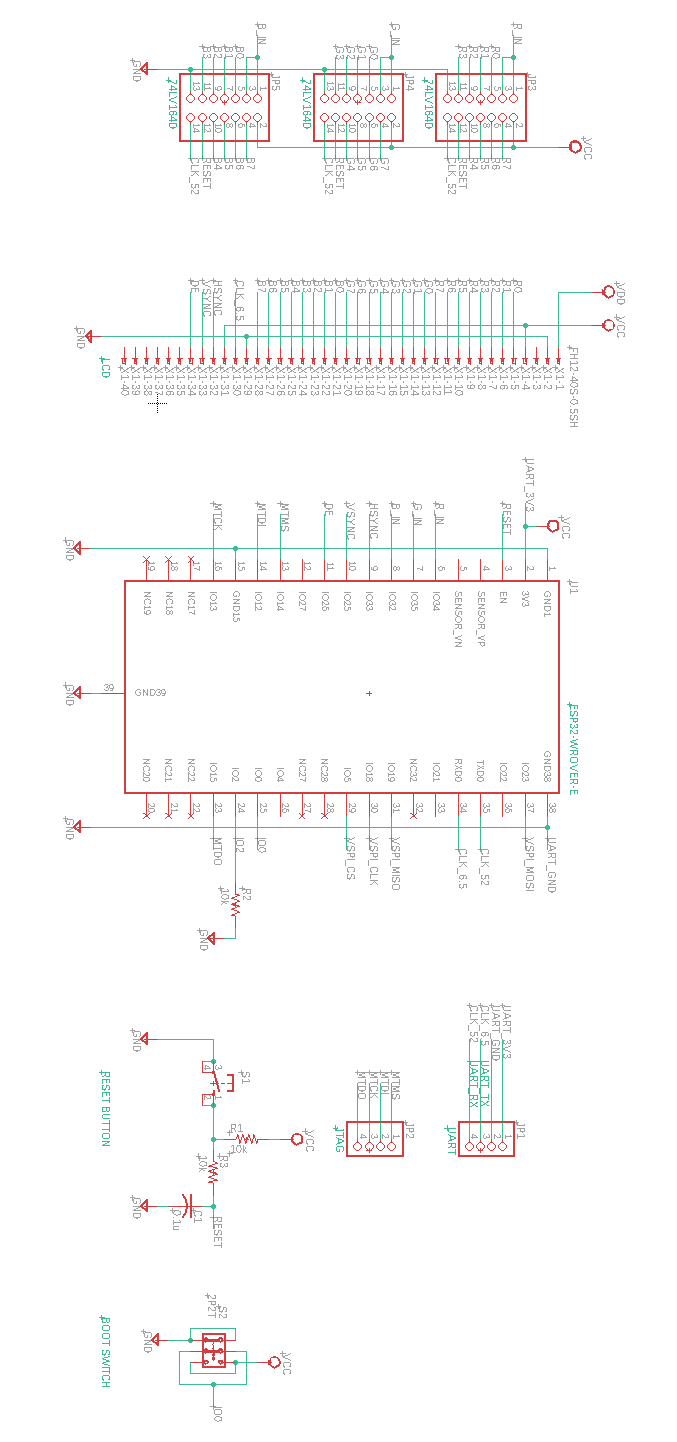
\includegraphics[height=0.86\textheight]{Comms_Display_Schem.png}
\end{figure}

\newpage
\section{Appendix C: Power Subsystems Schematic}



\newpage
\section{Appendix D: MCU Firmware Flow Diagram}



\end{document}
